%%%%%%%%%%%%%%%%%%%%%%%%%%%%%%%%%%%%%%%%%
% Beamer Presentation
% LaTeX Template
% Version 1.0 (10/11/12)
%
% This template has been downloaded from:
% http://www.LaTeXTemplates.com
%
% License:
% CC BY-NC-SA 3.0 (http://creativecommons.org/licenses/by-nc-sa/3.0/)
%
%%%%%%%%%%%%%%%%%%%%%%%%%%%%%%%%%%%%%%%%%

%----------------------------------------------------------------------------------------
%	PACKAGES AND THEMES
%----------------------------------------------------------------------------------------

\documentclass{beamer}

\mode<presentation> {

% The Beamer class comes with a number of default slide themes
% which change the colors and layouts of slides. Below this is a list
% of all the themes, uncomment each in turn to see what they look like.

%\usetheme{default}
%\usetheme{AnnArbor}
%\usetheme{Antibes}
%\usetheme{Bergen}
%\usetheme{Berkeley}
%\usetheme{Berlin}
%\usetheme{Boadilla}
%\usetheme{CambridgeUS}
%\usetheme{Copenhagen}
%\usetheme{Darmstadt}
%\usetheme{Dresden}
%\usetheme{Frankfurt}
%\usetheme{Goettingen}
%\usetheme{Hannover}
%\usetheme{Ilmenau}
%\usetheme{JuanLesPins}
%\usetheme{Luebeck}
%\usetheme{Madrid}
%\usetheme{Malmoe}
%\usetheme{Marburg}
%\usetheme{Montpellier}
%\usetheme{PaloAlto}
%\usetheme{Pittsburgh}
%\usetheme{Rochester}
%\usetheme{Singapore}
%\usetheme{Szeged}
\usetheme{Warsaw}

% As well as themes, the Beamer class has a number of color themes
% for any slide theme. Uncomment each of these in turn to see how it
% changes the colors of your current slide theme.

%\usecolortheme{albatross}
%\usecolortheme{beaver}
%\usecolortheme{beetle}
%\usecolortheme{crane}
%\usecolortheme{dolphin}
%\usecolortheme{dove}
%\usecolortheme{fly}
%\usecolortheme{lily}
%\usecolortheme{orchid}
%\usecolortheme{rose}
%\usecolortheme{seagull}
%\usecolortheme{seahorse}
%\usecolortheme{whale}
%\usecolortheme{wolverine}

%\setbeamertemplate{footline} % To remove the footer line in all slides uncomment this line
%\setbeamertemplate{footline}[page number] % To replace the footer line in all slides with a simple slide count uncomment this line

%\setbeamertemplate{navigation symbols}{} % To remove the navigation symbols from the bottom of all slides uncomment this line
}

\usepackage{graphicx} % Allows including images
\usepackage{booktabs} % Allows the use of \toprule, \midrule and \bottomrule in tables
\usefonttheme{serif}

%----------------------------------------------------------------------------------------
%	TITLE PAGE
%----------------------------------------------------------------------------------------

\title[Model validation]{Shallow water model} % The short title
\subtitle{Validation}% appears at the bottom of every slide, the full title is only on the title page

\author{Edgar Gago Carrillo} % Your name
\institute[ESEIAAT] % Your institution as it will appear on the bottom of every slide, may be shorthand to save space
{
Polytechnic University of Catalonia \\ % Your institution for the title page
\medskip
\textit{edgargc.upc@gmail.com} % Your email address
}
\date{\today} % Date, can be changed to a custom date

\begin{document}

\begin{frame}
\titlepage % Print the title page as the first slide
\begin{figure}
    \centering
    
\includegraphics[scale=0.05]{imagenes/logo.png}
\end{figure}
\end{frame}

\begin{frame}
\frametitle{Overview} % Table of contents slide, comment this block out to remove it
\tableofcontents % Throughout your presentation, if you choose to use \section{} and \subsection{} commands, these will automatically be printed on this slide as an overview of your presentation
\end{frame}

%----------------------------------------------------------------------------------------
%	PRESENTATION SLIDES
%----------------------------------------------------------------------------------------

%------------------------------------------------
\section{The model}
%------------------------------------------------

\subsection{Geometry} 
\begin{frame}{Geometry}

\end{frame}

%------------------------------------------------
\subsection{Matlab configuration}
\begin{frame}{Matlab configuration}

\end{frame}

%------------------------------------------------
\section{Validation of the model }
\subsection{Design conditions}
\begin{frame}{conditions}

\end{frame}

\subsection{Advective terms}
\begin{frame}{P2}

\begin{columns}[c]
	\column{.45\textwidth}
	\begin{figure}
		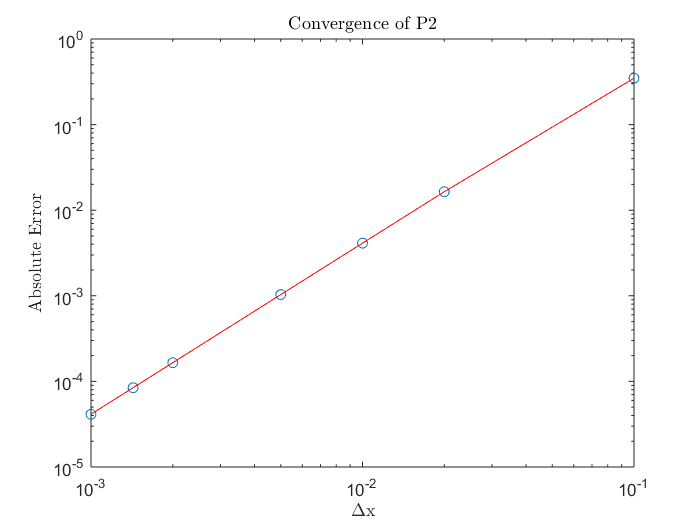
\includegraphics[scale=0.35]{imagenes/P2.png}
		\caption{Convergence of the advective term P1}
	\end{figure}
	
	\column{.4\textwidth}
	\begin{itemize}
		\item
	\end{itemize}
\end{columns}
\end{frame}

\begin{frame}{P1}
\end{frame}

\subsection{Mass conservation}
\begin{frame}{$\eta$}
\end{frame}
%------------------------------------------------

\section{Testing the model}

\subsection{Initial conditions}
\begin{frame}
\begin{columns}[c] % The "c" option specifies centered vertical alignment while the "t" option is used for top vertical alignment

\column{.45\textwidth} % Left column and width
\textbf{Heading}
\begin{enumerate}
\item Statement
\item Explanation
\item Example
\end{enumerate}

\column{.5\textwidth} % Right column and width
Lorem ipsum dolor sit amet, consectetur adipiscing elit. Integer lectus nisl, ultricies in feugiat rutrum, porttitor sit amet augue. Aliquam ut tortor mauris. Sed volutpat ante purus, quis accumsan dolor.

\end{columns}
\end{frame}

\subsection{First results}
\begin{frame}
\end{frame}

%------------------------------------------------
\section{Conclusions}
%------------------------------------------------
\begin{frame}
	
\end{frame}

%------------------------------------------------

\begin{frame}
\Huge{\centerline{Thnk you for your attention}}
\end{frame}

%----------------------------------------------------------------------------------------

\end{document}